% Eğer Tezinizi bu dosyada yazacaksanız "TEZİNİZİ BURADAN SONRA EKLEYİNİZ" bölümünden sonra ekeleyebilirsiniz. Özet ve Summary bölümleri /bolum klasörünün içindedir.


\documentclass[]{esogu}			% Optionlar boş olacak, şablonu kullanmak için
\usepackage{lipsum}				% Örnek tezde anlamsız metin yazmak için bu paket gerekli. Tezinizde bu bölümü silebilirsiniz.
\usepackage{atbegshi} % İçindekiler, şekiller ve çizelgelerde birinci sayfadan sonraki sayfalara devam yazmak için
\makeatletter
\newcommand{\AtBeginShipoutClear}{\gdef\AtBegShi@Hook{}}
\makeatother
\usepackage{pdfpages}
\usepackage{tikz}
\bibliography{kaynakca.bib}		% Kaynakça dosyası için Bunu Zotero, Mendeley, Endnote ya da CiteU gibi bir programla oluşturmanızı tavsiye ederim. Zotero hakkında bilgi http://makina.gmay.me/Bulutta/ adresindeki ekitapta mevcut.
\usepackage{listings}
\usepackage{color}

\definecolor{codegreen}{rgb}{0,0.6,0}
\definecolor{codegray}{rgb}{0.5,0.5,0.5}
\definecolor{codepurple}{rgb}{0.58,0,0.82}
\definecolor{backcolour}{rgb}{0.95,0.95,0.92}

\lstdefinestyle{mystyle}{
    backgroundcolor=\color{backcolour},
    commentstyle=\color{codegreen},
    keywordstyle=\color{magenta},
    numberstyle=\tiny\color{codegray},
    stringstyle=\color{codepurple},
    basicstyle=\footnotesize\ttfamily,
    breakatwhitespace=true,
    breaklines=true,
    captionpos=b,
    keepspaces=true,
    numbers=left,
    numbersep=5pt,
    showspaces=false,
    showstringspaces=false,
    showtabs=false,
    tabsize=2
}
\lstset{style=mystyle}


%%%%%%%KISALTMALAR%%%%%%%%%%%%%%%%%%%
%% Kısaltmalar için lütfen glossaries paketine bakınız.
\newglossarystyle{mylong3col}{%
  \setglossarystyle{long3colheader}%
  \renewcommand\entryname{Simge veya Kısaltma}
  \renewcommand\descriptionname{Tanım}
  \renewcommand{\pagelistname}{Sayfa Numarası}
  \renewenvironment{theglossary}%
    {\begin{longtable}[l]{@{}lp{0.5\hsize}p{0.3\hsize}}}%
    {\end{longtable}}%
}
%
%
\newacronym{OBEB}{OBEB}{Ortak Katların En Büyüğü}

\newacronym{AMBA}{AMBA}{Advanced Microcontroller Bus Architecture}
\newacronym{MEM-AP}{MEM-AP}{Memory Access Port}
\newacronym{DAP}{DAP}{Debug Access Port}
\newacronym{AP}{AP}{Access Port}
\newacronym{CSV}{CSV}{Comma Separated Values}
\newacronym{DP}{DP}{Debug Port}
\newacronym{LSB}{LSB}{Least Significant Bit}
\newacronym{I2C}{I2C}{Inter-Integreted Circuit}
\newacronym{ADC}{ADC}{Analog Digital Converter}
\newacronym{MCU}{MCU}{Micro Controller Unit}
\newacronym{SDK}{SDK}{Software Development Kit}
\newacronym{ICSP}{ICSP}{In Circuit-System Programming}
\newacronym{IDE}{IDE}{Integrated Development Environment}
\newacronym{SPI}{SPI}{Serial Perhiphal Interface}
\newacronym{SWD}{SWD}{Serial Write Debug}
\newacronym{HTML}{HTML}{Hyper Text Markup Language}
\newacronym{JS}{JS}{Java Scipt}
\newacronym{OKEK}{OKEK}{Ortak Katların En Küçüğü}
\newacronym{pi}{$\pi$}{$\pi$ sayısı}

%----------------------------------------------------------------------------------------
\begin{document}

\frontmatter %roma rakamları ile yazdırmak için
\title{Pau Thesis}
%-----Dış kapak Türkçe---------- Burayı değiştirmeyin
\begin{titlingpage*}
\begin{center}
\large
\textbf{\MakeUppercase{\uni}}

\vspace{1pc}
\textbf{\MakeUppercase{\fakulte}}

\vspace{1pc}
\textbf{\MakeUppercase{\bolum}}
\vspace{2pc}

%---------------bolum logosu-------------------------
	\begin{figure}[h]
	\centering
	
\includegraphics[width=0.25\textwidth]{gorseller/image1}
	\end{figure}
	\vspace{2pc}
  \Large
	\textbf{\unvan\space BİTİRME TEZİ}\\
  \vspace{1pc}							%12 punto boşluk ver
  \normalsize
\end{center}
\begin{framed}
\begin{center}
\textbf{GÜÇ ELEKTRONİĞİ TABANLI UYGULAMALARDA \\MİKROİŞLEMCİLERİN NETWORK ÜZERİNDEN PROGRAMLANMASI\\ VE VERİ AKTARIMI} %Daha toplu olmasi icin boyle yaptim
\vspace{1pc}

\yazar\\
\vspace{1pc}

\teslim\\
\vspace{1pc}

Tez Danışmanı:\hspace{10mm} \danisman
\end{center}
\end{framed}
\end{titlingpage*}

%---------------Tez kunyesi-----------------------

\begin{table}[]
\begin{tabular}{|l|l|}
\hline
\multicolumn{2}{|c|}{\textbf{TEZ KÜNYESİ}}      \\ \hline
1. ARŞİV NUMARASI    & 2. SAVUNMA TARİHİ \\
\hspace{10ex}       & \hspace{2ex}20 Mayıs 2019    \\ \hline
\multicolumn{2}{|l|}{4.TEZ BAŞLIĞI}    \\
\multicolumn{2}{|p{14cm}|}{\hspace{2ex}\tbaslik}\\ \hline
5.YAZAR              & 6.TEZ DANIŞMANI \\
\hspace{2ex}\yazar   & \hspace{2ex}\danisman  \\ \hline
\multicolumn{2}{|l|}{6.ÖZET}           \\
	\multicolumn{2}{|p{14cm}|}{\hangindent=2ex\hspace{2ex}1900’lü yıllarda serüvenine başlayan güç elektroniği ve uygulamarı
yarıiletkenler ve sayısal elektronik ile büyük hız kazanmıştır. Güç elektroniği
uygulamarında gerekli olana tetikleme sinyali, giriş akımı, gerilimi; çıkış
akımı, gerilimi değerlerin ölçümesi gibi gereksinimleri mikrokontorolcüler
karşılamaktadır.

Günümüzün popüler ve hızla gelişen konularından olan Nesnelerin İnterneti
(IoT) ile cihazlar bir internete erişim sağlayıp diğer cihazlar ile iletişim
içeresinde bulunmaktadır. Bu gelişmeler, güç elektroniği uygulamarında
kullanılan mikrodenetleyicilerin uzaktan programlanması ve denetleyicilerin
topladığı verilerin internete aktarılması gibi yeni gereksinimleri ardında
getirmiştir.
}              \\ \hline
7.ANAHTAR KELİMELER & 8.SAYFA SAYISI   \\
	ESP8266, SWD, ARM, Network & 22 \\
\hspace{10pt}             & \hspace{10pt}  \\ \hline
\end{tabular}
\end{table}

\clearpage
%----------Onay-------------------------------------
\thispagestyle{empty}
%\begin{center}
%\large
%\textbf{\MakeUppercase{\tbaslik}}\\
%\vspace{1pc}
%\yazar\\
%\vspace{1pc}
%\teslim\\
%\vspace{2pc}
%\end{center}
%\vspace{2pc}
%\normalsize
%Bu çalışma, jürimiz tarafından Elektrik-Elektronik Mühendisliği Bölümü’nde Lisans
%Bitirme Tezi olarak kabul edilmiştir.
%
%\vspace{20mm}
%
%\noindent \textbf{Tez Danışmanı:\hspace{5ex}\danisman}
%
%\hspace{20ex}\uni
%
%\hspace{20ex}\fakulte
%
%\hspace{20ex}\bolum
%\vspace{1pc}
%
%\noindent \textbf{Üye:\hspace{15ex}\jbir}
%
%\hspace{20ex}\uni
%
%\hspace{20ex}\fakulte
%
%\hspace{20ex}\bolum
%\vspace{1ex}
%
%\noindent \textbf{Üye:\hspace{15ex}\jiki}
%
%\hspace{20ex}\uni
%
%\hspace{20ex}\fakulte
%
%\hspace{20ex}\bolum
%\vspace{1pc}
%
%\noindent \textbf{Onaylayan:\hspace{9ex}\onay}
%
%\hspace{20ex}\uni
%
%\hspace{20ex}\fakulte
%
%\hspace{20ex}\bolum
\includepdf{tezSon.pdf}
\newpage


%-------------------Şekiller ve Çizelgeler Dizini----------------
\renewcommand{\listfigurename}{ŞEKİLLER LİSTESİ}
\renewcommand{\listtablename}{TABLOLAR LİSTESİ}

\setlength\beforechapskip{-\baselineskip}

\normalsize

%Özette tez çalışmasının amacı, kapsamı, kullanılan yöntemler ve varılan sonuçlar açık ve öz olarak belirtilmeli, bunlar alt başlıklar altında sunulmamalıdır.  Özetin uzunluğu 250 kelimeyi geçmemelidir. 

%Summary sayfasının içeriği ve düzeni tümüyle Özet sayfasının aynı olmalı ve (vii) ile numaralanmalıdır.

%Özet ve Summary’nin altına anahtar kelimeler/keywords yazılmalıdır.  Konu literatürde hangi kelimelerle geçiyorsa anahtar kelime olarak bu kelimeler kullanılmalıdır.

\chapter{ÖZET}

\lipsum[1]
\chapter{TEŞEKKÜR}

Öncelikle, yetişmemde en büyük pay sahibi olan aileme teşekkür etmeyi bir vazife olarak görüyorum.
Bu çalışma süresince beni yönlendiren ve yardımlarını benden esirgemeyen tez danışmanım sayın Doç. Dr. Selami Kesler'e teşekkürlerimi sunarım. Ayrıca tez çalışmamı hazırlamamda, çeşitli konularda yardımlarından dolayı Abdülkadir ABAKAY'a ve Raşit EVDÜZEN'e teşekkürlerimi sunarım.
\\\\\\
\textbf{Çağatay YILMAZ}


\AtBeginShipout{\protect\chapter*{İÇİNDEKİLER (Devam)}}
\tableofcontents*
\AtBeginShipoutClear
\newpage
\AtBeginShipout{\protect\chapter*{ŞEKİLLER LİSTESİ (Devam)}}
\listoffigures
\AtBeginShipoutClear
\newpage
\AtBeginShipout{\protect\chapter*{ÇİZELGELER LİSTESİ (Devam)}}
\listoftables
\AtBeginShipoutClear
\clearpage

\clearpage
%\printglossary[style=mylong3col, type=\acronymtype, title=Simgeler ve Kısaltmalar Listesi, toctitle=SİMGELER VE KISALTMALAR LİSTESİ]
\textbf{SİMGELER VE KISALTMALAR LİSTESİ}

\begin{table}[h]
\begin{tabular}{l l}
	\textbf{AMBA:	} & Advanced Microcontroller Bus Architecture \\
	\textbf{MEM-AP:	} & Memory Access Port \\
	\textbf{DAP:	} & Debug Access Port \\
	\textbf{AP:	} & Access Port \\
	\textbf{DP:	} & Debug Port \\
	\textbf{LSB:	} & Least Significant Bit \\
	\textbf{I2C:	} & Inter-Integreted Circuit \\
	\textbf{ADC:	} & Analog Digital Converter \\
	\textbf{MCU:	} & Micro Controller Unit \\
	\textbf{SDK:	} & Software Development Kit \\
	\textbf{ICSP:	} & In Circuit-System Programming \\
	\textbf{IDE:	} & Integrated Development Environment \\
	\textbf{SPI:	} & Serial Perhiphal Interface \\
	\textbf{SWD:	} & Serial Write Debug \\
	\textbf{HTML:	} & Hyper Text Markup Language \\
	\textbf{JS:	} & Java Scipt \\
\end{tabular}
\end{table}
%\printglossary[style=mylong3col, type=\acronymtype]
\clearpage


\mainmatter %arap harfleri ile yazdırmak için
% AltBölüm numaralaması
\setcounter{secnumdepth}{5} % 5 derine kadar numara ver.
%---------TEZİNİZİ BURADAN SONRA EKLEYİNİZ-----------------



\chapter{GİRİŞ}

Güç elektroniği serüvenine 1900'lü yıllarda güç elektroniği doğru akım motorlarının hız kontrolü ile başlamıştır.
Elektron tüpleri ile teorik çalışmalar yapılmıştır, fakat uygulamaya sokulmamıştır.
1950 yılında yarıiletkenler, 1960 yılında tristörler, 1980 yılında sayısal elektronik ve
mikroişlemcilerin geliştirilmesi ile güç elektroniği otomotiv, endüstri, ulaşım araçları gibi bir çok sektörde faailiyet
göstermektedir.

Güç elektroniğinde mikrodenetleyiciler, yarıiletkelerin ihtiyaç duyduğu tetikleme sinyallerinin oluştrulması,
akım ve gerilim değerlerin okunması gibi ihtiyaçları karşılmaktadır.

İletişim altyapısını ve teknik gelişmeler sonucu günümüzün popüler konusu olan nesnelerin interneti ile,
güç elektroniği uygulamarında kullananılan mikrodenetleyicilerin uzaktan erişim ile yazılımlarının ve paremetrelerinin
güncellenmesi, denetleyici tarafıdan okunan değerlerin görüntülenmesi gibi ihtiyaçlar ortaya çıkmıştır.

Bu çalışmada belirtilen ihtiyaçları karşılamak amacıyla; güç elektroniğinde sıklıkla kullanılan ARM tabanlı mikrodenetleyiciler
için programlamama ve veri aktarımı sağlamak üzere ESP8266 mikroişlemcisi kullanıldı.
ESP8266 hedef denetleyicinin debug portu olan \acrfull{SWD} portuna bağlı olacak ve buradan işemcinin
registerlarına ve hafıza birimlerine erişecek. Aynı zamanda web server olarak çalışacak ve kullanıcı ile hedef
işlemci arasında arayüz oluşturacaktır.



				% Metni dosyadan çağırmak için örnek
\chapter{Mikrodenetleyicilerin Programlanması}

\acrfull{mcu}, içerisinde hafıza birimleri(RAM, ROM, Flash), giriş/çıkış birimleri olan programlanabilen entegrelerdir.
%%-_--_-_-_-_-_-_-_-_-_-_-_-_-_-_-_-Denetleyici Resimi Koy-_-_-_-_-_-_-_-_-_-_-_-_-_-_-_-_-_-_-_-_-_-_-_

Mikrodenetleyicilerin programlanması, bilgisayar oramında yazılmış olan kodun hedef işlemci için derlenmesi
ve derleme sonucu ortaya çıkan makina kodlarının bir şekilde denetleyicinin hafıza birimine aktarılması olarak açıklanır.
Mikrodenetlecilerden önce mikroişlemciler ile kurulan sistemlerde programlama işlemi, hafıza biriminin sistenden ayırarak
bir programlacı yardımı ile makina kodlarının aktarılmasıyla gerçekleşiyordu. Mikrodenetleyicilerde hafıza birimi entegre
içinde gömülü olarak bulunduğu için programalama işlemini bu şekilde gerçeklemek münkün değildir.

Günümüzlde mikrodenetleyiciler \acrfull{ICSP} olarak adlandırlan programlayıcılar ile programlanmaktadır. \arcshort{ICSP} programlayıcılar,
denetleyicinin programlama pinleri aracılıyla işlemcinin hafıza birimine erişim sağlayarak makina kodlarını aktarır.
Bu işlem ARM tabalı mikrodenetleyicilerde \acrfull{SWD} debug portu ya da JTAG portu ile gerçekleştirmektedir.

ARM Debug Arayüzünde

\chapter{Tez Çalışmasında Kullanılan Araçlar ve Cihazlar}

Bu çalışmada hedef cihazın, kablosuz ağ üzerinde programlanması ve veri aktarınımı sağlamak amacıyla sunucu cihaz olarak, Esp8266 mikrodenetleyicisi kullanılmıştır.
Hedef cihaz ile, sunucu cihaz arasında iletişimi sağlayan \acrfull{SWD} protokolünün işleyişini çözümlemek ve sunucu cihaz için yazılan kodların test sırasında işlemleri
incelemek amacıyla Lojik Analizör kullmılmıştır.

Hedef cihaz olarak ST firmasının ürettiği geliştirme kartı olan Discovery ailesinden, STM32F072 geliştirme kartı şeçilmiştir.

\section{ESP8266 Mikrodenetleyicisi}

ESP8266, Espressif firmasının geliştirdiği  mikrodenetleyicidir. Esp8266; 32 bitlik Tensilica mimarisine sahip işlemci, genel amaçlı çevre birimleri,
RF balun, güç amplifikatör devreleri, düşük gürültülü amplifikatör devreleri, filtreler ve güç yönetim modullerini küçük bir entegre paket halinde sunmaktadır. Aynı zamanda, 2.4 GHz Wi-Fi (802.11 b/g/n),
16 adet genel amaçlı giriş çıkış portu, \acrfull{I2C} portu, \acrfull{SPI} portu, 10 bitlik \acrfull{ADC}, 80 KiB  RAM mevcuttur. Harici olarak 8 MB'ta kadar SPI flash hafıza birimi
kullanılabilmektedir.


\begin{figure}[h]
\centering
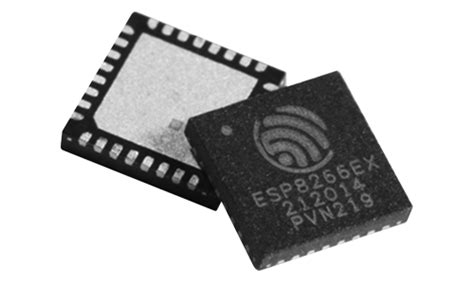
\includegraphics[width=\textwidth]{gorseller/esp8266ex}
\caption{ESP8266 Mikrodenetleyicisi.}\label{fig:esp8266ex}
\end{figure}

Geliştirme ortamı olarak, ESP8266 işlemcisi için kodların yazımında text editör olan VIM ve yazılan kodların derlenmesi, ESP8266 aktarılması için Arduino \acrfull{IDE}'si kullanılmıştır.
Espressif firmasının ESP8266 denetleyicisi için oluşturduğu \acrfull{SDK}, derleme zorluklarından ve derleme süreçlerinin uzun sürmesinden olayı Arduino IDE tercih edilmiştir.

ESP8266 denetleyicisi, hem SWD protokolü için sunucu cihaz hem de kullanıcı arayüzü olarak HTTP server olarak çalışacaktır. Kullanıcı arayüzünün platformdan ve işletim sisteminden bağımsız olması ve kurulum gerektirmediği için HTML ile web sayfası olarak tasarlanmıştır.

\section{Lojik Analizör}

Lojik analizör sayısal veri yolu üzerindeki işaretlerin gözlemlenmesi, ikilik tabanda oluşan kodları çözümlenmesini sağlayan mantıksal cihazdır. Bu çalışmada kullanılan lojik analizör Şekil \ref{fig:lojikAna}'de verilmiştir.

\begin{figure}[h]
\centering
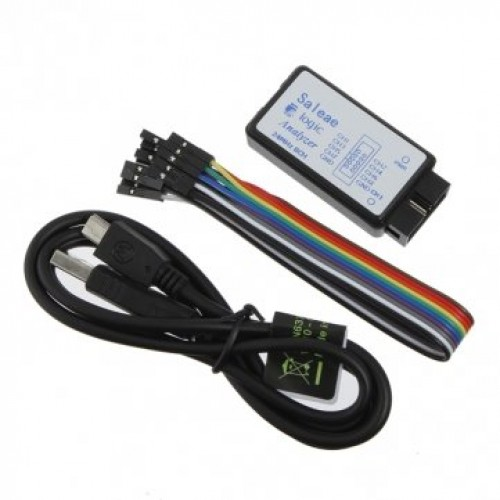
\includegraphics[width=0.7\textwidth]{gorseller/lojikAna}
\caption{Çalışmada Kullanılan Lojik Analizör}\label{fig:lojikAna}
\end{figure}

SWD protokolünü çözümlemek ve işlem sırasını çıkartmak için lojik analijör kullanılmıştır. Hedef cihaz olarak seçilen STM32F072 Discovery kartı üzerinde bulunan ST-Link SWD programlayıcısının, denetleyiciyi programlama sırasında lojik analizör ile protokol verilerini kaydederek protokol çözümlemesi yapıldı. Lojik analizörün arayüzünde dahili olarak bulunan SWD çözümleyici ile sistemin çalışması kontrol edildi.

\begin{figure}[h]
\centering
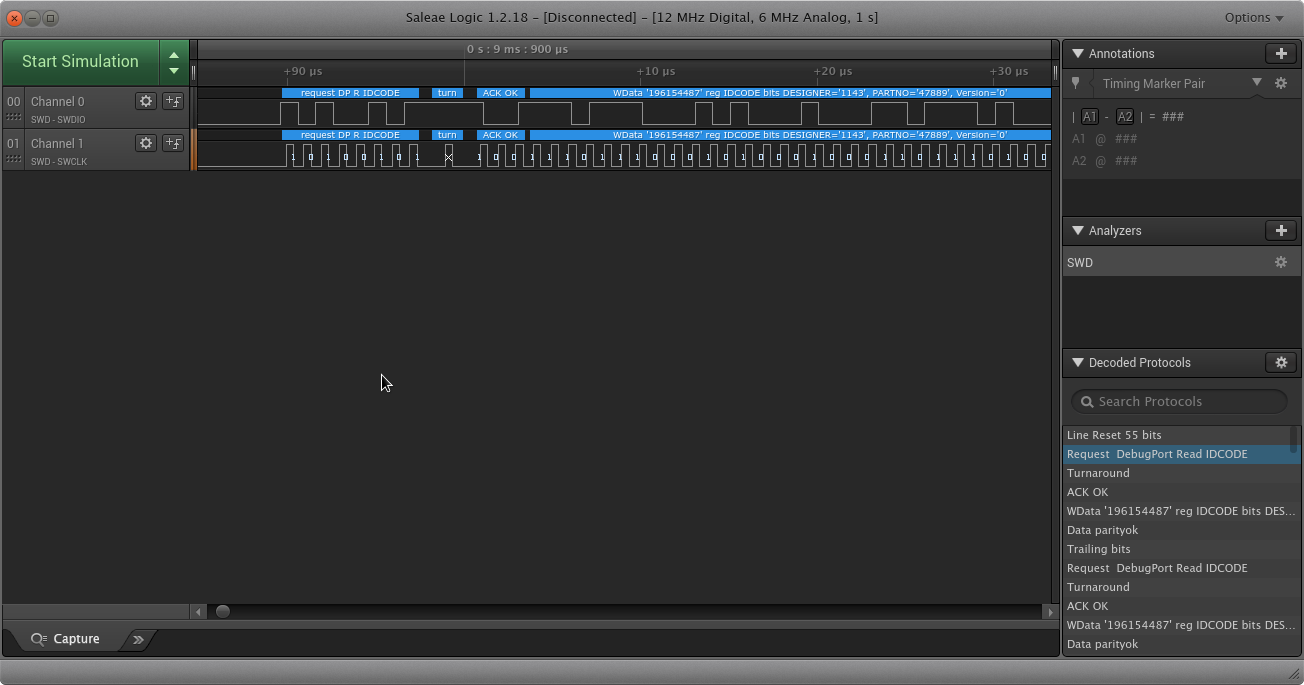
\includegraphics[width=\textwidth]{gorseller/lojikOut}
\caption{Örnek Lojik Analizör Çıktısı}\label{fig:lojikOut}
\end{figure}


Protokolün ve ardışık işlemlerin tanımlanması sonucunda, ESP8266 ile yapılan SWD uygulamasının testi sırasında lojik analizör kullanıldı.

\section{STM32F072 Discovery Kartı}

Elektronik ve yarıiletken komponent üreticisi olan STMicroelectronics tarafıdan geliştirilen, ARM Cortex-M0 mikroişlemcisine sahip olan STM32F072 mikrodenetleyicisi hedef cihaz olarak seçilmiştir. Ancak ARM tarafıdan geliştirilen SW-DP ve SWD, çoğu ARM işlemciler için ortak olduğu için bu tez çalışması için seçilen hedef cihaz dışında diğer ARM tabanlı mikrodenetleyiler bu çalışma kapsamı içindedir.

\begin{figure}[h]
\centering
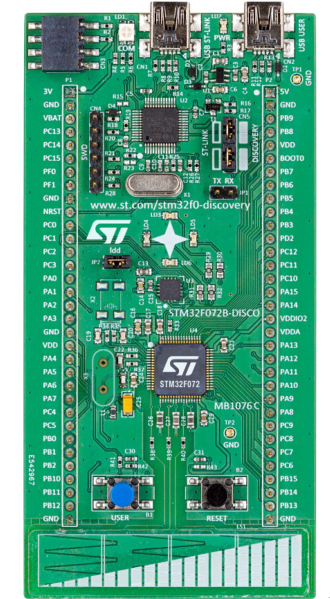
\includegraphics[width=0.4\textwidth]{gorseller/stmDisco}
\caption{STM32F072 Discovery Geliştirme Kartı.}\label{fig:stmDisco}
\end{figure}

STM32F0 Discovery kartı üzerinde, STM32F072RBT6 mikrodenetleyicisi, ST firmasının geliştirdiği jiroskop, liner dokumatik sensörü, buton, LED ve ST-LINK/V2 bulunmaktadır. STM32F072 kartı için test kodu; ST firmasının geliştirdiği STM32CUBEMX paket programı ile sistem konfigürasyon kodları oluşturulup, 'arm-none-eabi-gcc' derleyicisi ile derlenme işlemi yapılmıştır. Test kodu, STM32F072 Discovery kartı üzerinde bulunan 4 tane ledin yanıp sönmesi üzerine yazılmıştır. Farklı sıra ve süre ile oluşturulmuş test yazılımlar, sunucu cihazın programlayıcı özelliğinin test sırasında kullanılacaktır.




\chapter{Seri Hat Hata Ayıklama Portu (SWD-DP)}

%Serial Wire Debug (SWD) is a 2-pin (SWDIO/SWCLK) electrical alternative JTAG interface that has the same JTAG protocol on top.
%SWD uses an ARM CPU standard bi-directional wire protocol, defined in the ARM Debug Interface v5.
%This enables the debugger to become another AMBA bus master for access to system memory and peripheral or debug registers.
%
%
%
%The Debug Access Port (DAP) is split into two main control units. The Debug Port (DP) and the Access Port (AP),
%and the physical connection to the debugger is part of the DP. The DAP supports two types of access,
%Debug Port (DP) accesses and Access Port (AP) accesses. External device to communicate directly with Serial Wire Debug Port
%(SW-DP) over SWDIO/SCLK pins. And SW-DP in turn can access one or several Access Ports (APs) the give access to the rest of
%the system. The MEM-AP is important AP which provide a way to access all memory
%and peripheral registers residing on the internal AHB/APB buses.

\acrfull{SWD}, iki pin bağlantısı ile, JTAG arayüzüne alternatif olarak, pin kısıtlaması olan mikrodenetleyiciler için geliştirilmiştir.
ARM Hata Ayıklama Arayüzü v5 ile tanımlanmış olan SWD, hata ayıklma portu ile ARM işlmecisinin \acrshort{AMBA} veriyoluna erişim sağlar. Bu sayade
işlmecinin sistem hafıza birimlerine, çevre birimlerinin ve sistem yazmaçlarına erişim sağlamaktadır.

\acrfull{DAP}, Hata Ayıklma Portu (\acrshort{DP}) ve Erişim Portu (\acrshort{AP}) olmak üzere iki ana kontrol birimine arılmıştır. ARM işlecisine erişmek isteyen cihaz
Seri Hat Hata Ayıklama Portu'nun SWDIO ve SCLK pinlerine fiziksel olarak bağlanaması gerekmektedir. SWD-DP ile sistemin geri kalan erişim ve hata ayıklama portuna erişim
sağlamak mümkündür. \acrfull{MEM-AP}, dahili AHB/APB veriyollarına, hafıza elemanlarına ve çevre birimlerine erişim sağlayabilen en önemli erişim portudur.

%---------------------------------- resim koy------------------------------------------------------------------

\section{SWD Protokolü}

SWD protokülü iki pin üzerinden (SWDIO-SCLK) hedef işlemcinin hata ayıklama portuna erişim sağlamaktadır. SWD'nin kullandığı iki pinden birisi olan SWDIO pini iki yönlü hat olup
veri alış-verişinin yapıldığı veri hattır. Diğer pin olan (SCLK), iletişim için gerekli olan saat (clock) sinyalini barındıran sinyal hattıdır. Saat sinyali hattı servis sunucusu tarafından
sağlanır.

\section{SWD Baglatı ve Reset}

Hedef cihazın Hata Ayıklama Portu'na fiziksel olarak bağlanıldıktan sonra, SWDIO pini lojik 1 seviyesine çekilerek SCLK hattından en az 50 puls verilmelidir. Bu işleme hat sıfırlama (Line Reset) adı verilir.
ARM işlemcisinide bulunan SWD Hata Ayıklama portunu seçmek için hat sıfırlama işleminden sonra onaltı bitlik "0xE79E" verisi, veri hattından saat sinyali ile birlikte gönderilir. Ardından
işlemcinin 'IDCODE' yazmacı okunur. Eğer okunan yazmaç değeri doğru ise SWD protoklü başarılı bir şekilde başlamış demektir.

\section{Veri Göndeme ve Alma Süreçleri}

SWD protokolü kullanarak . Bunlar;
\begin{itemize}
	\item İstek Fazı: Servis Sunucusu 8 bitlik istek paketini hedef cihaza gönderir.
	\item Doğrulama Fazı: Hedef cihaz 3 bitlik doğrulama kodunu servis sunucusuna gönderir.
	\item Veri Fazı: İstek fazında bulunan okuma-yazma isteğine bağlı olarak hedef cihaz yada sunucu cihaz 33 bitlik veriyi veri hattından gönderir.
\end{itemize}

%---------------------------- RESIM KOY pulsler ve data olan----------------------------------------------------------------

\subsection{İstek Fazı}

\subsubsection{DEneme}




\chapter{ESP8266 İle SWD Protokolü Uygulaması}

Bu bölümde, ESP8266 ile SWD protoktolü için sunucu cihaz yapılacaktır. C++ programlama dili ile oluşturulan kodlar ESP8266 için derlenecektir. Bu bölümde [2]'de belirtilen çalışmadan yararlanılmıştır.

SWD protokolünde bulunan üç faz (istek, doğrulama, veri) temelde verinin tek pin (SWDIO) üzerinden saat sinyali ile birlikte, kaydırılarak okunması yada yazılması ile gerçekleştirilir. Burada dikkat edilmesi gereken nokta SWDIO pinin okuma sırasında giriş, yazma sırasında çıkış olarak ayarlanmasıdır.


\section{SWD İstek Verisinin Oluştrulması}

Bir önceki bölümde istek fazı 8 bit uzunluğundaki isteğin hedef cihaza aktarılması olarak bahsetmiştik. Bu istek verisinin öncelikle oluşturulması gerekmektedir. Bu işlemi gerçekleştiren 'packHeader()' C++ kodu Şekil \ref{fig:packHeader} verilmiştir.

\begin{figure}[h]
\centering
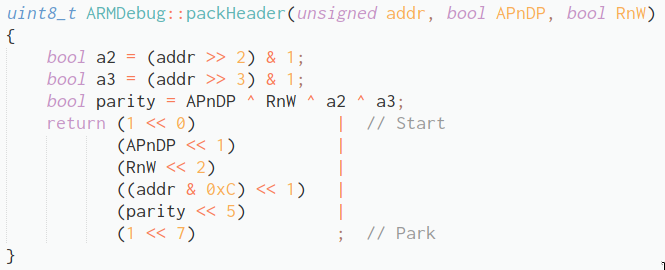
\includegraphics[width=\textwidth]{gorseller/packHeader}
\caption{packHeader() Fonksiyonu}\label{fig:packHeader}
\end{figure}


\section{Verinin Okunması ve Yazılması}

İstek fazının ardından gelen doğrulama ve veri fazı tek hat üzerinden yapılan okuma/yazma işlemidir. SWDIO pini üzerinden okuma işlemini gerçekleyen kod parçası Şekil \ref{fig:wireRead}'de gösterilmiştir. Şekilde gösterilen fonksiyonda bir tane paremetre almaktadır. Bu paremetre okunacak olan verinin bit sayısını temsil etmektedir.
\clearpage
\begin{figure}
\centering
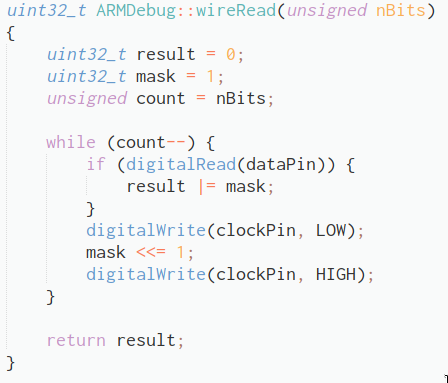
\includegraphics[width=0.6\textwidth]{gorseller/wireRead}
\caption{Okuma İşlemi için C++ Fonksiyonu}\label{fig:wireRead}
\end{figure}

Okunacak bit sayısı kadar tekrarlanan bir döngü içerisinde; SWDIO pini dijital olarak okunur, eğer değer lojik '1' ise sonuç ile maskeleme değişkeni lojik veya (or) işlemine sokulur. Eğer lojik '0' ise maske bir sola kaydırma işlemi yapılır. Döngü sonunda elde edilen sonuç fonksiyon çağrısına geri dönüş yapılır.

Tek pin üzerinde yazma işlemi için oluşturan C++ fonksiyon Şekil \ref{fig:wireWrite}'de gösterilmiştir. Yazma fonsiyonun iki adet parametre almaktadır. Bu parametrelerden biri yazılacak olan veriyi diğer ise verinin kaç bitlik veri olduğunu temsil etmekedir. Yazma işlemi; verinin \acrfull{LSB} öncelikli olarak aktarılması için, 1 ile (0b...00001) maskelenip pine çıkış olarak yazılması ve ardından verinin bir bit sağa kaydırılması, bit sayısı kadar tekrarlamasından oluşan döngüdür.


\begin{figure}[h]
\centering
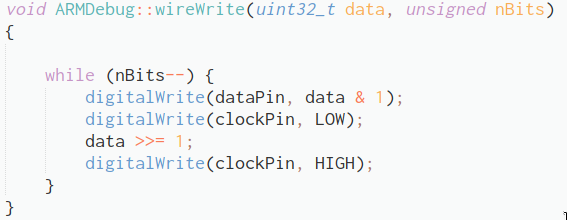
\includegraphics[width=\textwidth]{gorseller/wireWrite}
\caption{Yazma İşlemi için C++ Fonksiyonu}\label{fig:wireWrite}
\end{figure}

Okuma ve yazma fonksiyonları SWD protokolünde bulunan bütün fazlar için ortaktır. İstek fazında 8 bitlik veri yazma işlemi, doğrulama fazında 3 bitlik veri okuma işlemi ve veri fazında hem okuma hem de yazma işlemi yapılır.

Her fazın ardından gelen hat yön değişim periyodu temelde sunucu cihazda SWDIO pini olarak belirlenen pinin giriş yada çıkış olarak ayarlanmasıdır. SWDIO pini istek fazından önce çıkış, doğrulama fazıdan önce giriş, veri fazından önce eğer okuma yapılacak ise hat değişim periyodu uygulanmaz, yazma yapılacak ise hat çıkış olarak ayarlanmalıdır. Hat değişim periyodunu gerçekleyen C++ fonksiyonu Şekil \ref{fig:turnaround}'de verilmiştir.


\begin{figure}[h]
\centering
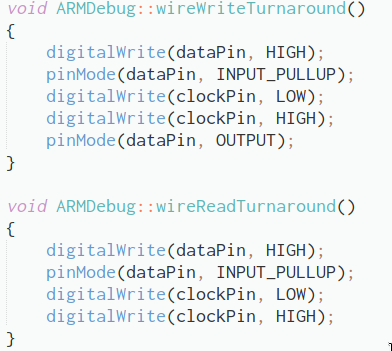
\includegraphics[width=0.7\textwidth]{gorseller/turnaround}
\caption{Yazma ve Okuma İşlemi İçin Hat Yön Değişim Periyodu}\label{fig:turnaround}
\end{figure}


\section{Line Reset}

Bir önceki bölümde SWD bağlantı, reset ve SW-DP portunun şeçimi için gerekli olan işlem sıralarından basettik. Bu işlem sıraları için yazılmış olan kodlar yukarıda belirtilen fonsiyonlar ile gerçekleştirilmiştir. Örnek olarak Şekil \ref{fig:lineReset}' de gösterilmektedir.
\clearpage

\begin{figure}[h]
\centering
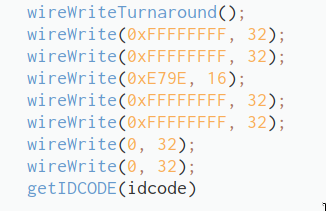
\includegraphics[width=0.7\textwidth]{gorseller/lineReset}
\caption{Yazma ve Okuma İşlemi İçin Hat Yön Değişim Periyodu}\label{fig:lineReset}
\end{figure}

Line reset işlemi için; en az 50 periyotluk '1' verisinin, SW-DP portunun şeçimi için gerekli olan kod '0xE79E' ve tekrar en az 50 bitlik '1' verisi yazılması gerekiyor. 50 bitlik '1' verisi için iki tane 32 bititlik '1' (0xFFFFFFFF) yazılmıştır. Şekilde gösterilen 'getIDCODE()' satırı, protokolün gerekliliği olan fonksiyon çağrısıdır.


\chapter{HTML ile Kullanıcı Arayüzü Tasarımı}

Kullanıcı arayüzü, \acrshort{HTML} ile web sitesi olarak tasarlandı. SWD protokolü için kullandığımız sunucu cihaz, aynı zamanda web sunucu olarak çalışacak. Yerel kablosuz ağa bağlı olan ESP8266, ip adresini RS232 portundan kullanıcıya bildirmektedir. Tarayıcı aracılığıyla bu ip adresine istek yapıldığında ESP8266 ilgili HTML sayfasını cevap olarak gönderir. Aynı zamanda HTTP isteğine bağlı olarak belirli betiği çalıştırarak SWD protokolü gerçekleştirir.

 ile oluşturulan statik sayfaları dinamik hale getirmek için \acrfull{JS} kullanıldı. JS tarayıcı tarafından çalıştırılan bir Java betiğidir. Bu çalışmada, JS ile sayfayı yenilemeden istenilen sayfa içeriğinin değiştirlmesi ve gerçek zamanlı grafik çizimi gibi uygulamar yapıldı.



\section{ESP8266 ile Web Sunucu}

Kullanıcı arayüzü için ESP8266 cihazını HTTP sunucu olarak çalıcaktır. ESP8266 için yazılmış Arduino kütüphaneleri ile sunucu kurulumu daha kolay gerçekleştirilmektedir.

HTTP (Hyper Text Transfer Protocol), internet sunucu ile kullanıcı arasındaki bilgilerin nasıl akracağını belirten kuralları ve yöntemleri belirten protokoldür. Http 4 fazdan meydana gelir. Bunlar;

\begin{itemize}
	\item \textbf{Bağlantı:} Web sunusuna bağtıntı kurulması.
	\item \textbf{İstek:} İsteğin web sunucusundan istenmesi.
	\item \textbf{Cevap:} İsteğe bağlı olarak sunucu tarafında dosyanın servis edilmesi.
	\item \textbf{Bağlantının kesilmesi:} Sunucu ile kullanıcı arasında yapılan bağlantının kesilmesi.
\end{itemize}

ESP8266 bulunduğu ortamdaki belirlenen kablosuz ağa bağlanacak ve web sunu servisi başlatacaktır. ESP8266 cihazına yapılan HTTP istekleri doğrultusunda, belirlen cevapları kullanıcıya döndürecektir.

ESP8266 ile yapılan örnek web sunucu kodları Şekil \ref{fig:webServer}'da gösterilmiştir.
\clearpage
\begin{figure}[h]
\centering
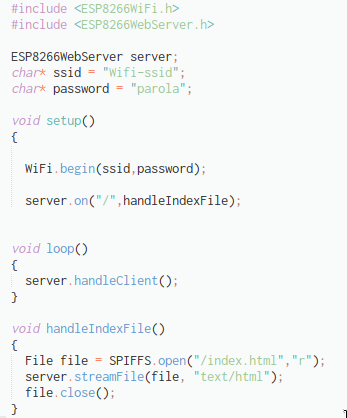
\includegraphics[width=0.7\textwidth]{gorseller/webServer}
\caption{ESP8266 ile Web Sunucu Kodları}\label{fig:webServer}
\end{figure}

Kodlarda bulunan "ssid" ve "password" değişkenleri bağlanılacak olan Wİ-Fİ ağının adını ve şifresini tutmaktadır. Bu tutulan değişkenler "WiFi.begin()" fonksiyonunda kullanılarak kablosuz ağa bağlanır. Bağlatı kurulduktan sonra "server.on("/", handleIndexFile)" satırı ile, kullanıcı tarafıdan gelen isteği "handleIndexFile" işleyici fonsiyonuna yönlendirir. Yönlendilen fonksiyon, ESP8266 dosya sistemi içerisinde bulunan "index.html" adındaki dosyayı kullanıcıya sunar.

Sunucuya bir istek yaptığında sunucu ilgili işleyici fonksionunu çağırır. İşyeci fonsiyonun isteğe bağlı olarak iki görevi üstlenmiştir. Bu görevler; ilgili dosyanın servis edilmesi ya da belirlenen betiğin çalıştırılmasıdır.


\chapter{SONUÇLAR VE ÖNERİLER}

Basit iki terimle \acrfull{OBEB} ve \acrfull{OKEK} kısaltmaları anlatabiliriz. İster kısaltmasını \acrshort{OBEB}, isterseniz de uzun açılımını \acrlong{OKEK} yazdırabilirsiniz. Bunu yapabilmek için dosyanın başında terimleri tanımlamanız gereklidir. İsterseniz matematik terimlerini de, örneğin \acrshort{pi} böyle tanımlayabilirsiniz. Uzun uzun \acrfull{pi} yazmanız gerekmez. 

Teorem yazmak isterseniz:
\begin{theorem}[Öklid]
 İki noktadan bir ve yalnız bir doğru geçer.
\end{theorem}

İspat yazmak isterseniz:
\begin{ispat}[Tezin en önemli ispatı]
x=10
\end{ispat}
\lipsum[1-2]
\begin{figure}[h]
\centering
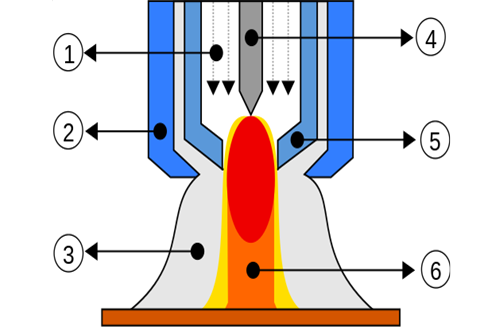
\includegraphics[width=\textwidth]{gorseller/ptaTorc}
\caption{PTA Torç}\label{fig:PtaTorc1}
\end{figure}
\lipsum[1-2]
\begin{table}
\centering
\caption{Deneme Tablosu.}\label{tab:den1}
\begin{tabular}{|l|l|l|}
\hline
sıra   & sayı   & toplam \\ \hline
1      & 2      & 3      \\ \hline
Kelime & deneme & son    \\ \hline
\end{tabular}
\end{table}


\section{Sonuçlar ve Öneriler Birinci Derece Başlık}
\lipsum[1-2]
\begin{figure}[h]
\centering
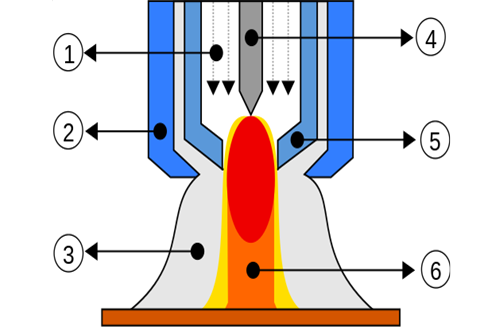
\includegraphics[width=\textwidth]{gorseller/ptaTorc}
\caption{PTA Torç}\label{fig:PtaTorc1}
\end{figure}
\lipsum[1-2]
\begin{table}
\centering
\caption{Deneme Tablosu.}\label{tab:den1}
\begin{tabular}{|l|l|l|}
\hline
sıra   & sayı   & toplam \\ \hline
1      & 2      & 3      \\ \hline
Kelime & deneme & son    \\ \hline
\end{tabular}
\end{table}
Teorem yazmak isterseniz:
\begin{theorem}[Öklid]
 İki noktadan bir ve yalnız bir doğru geçer.
\end{theorem}

İspat yazmak isterseniz:
\begin{ispat}[Tezin en önemli ispatı]
x=10
\end{ispat}

\subsection{Sonuçlar ve Öneriler ikinci derece başlık}
\lipsum[1-2]
\begin{figure}[h]
\centering
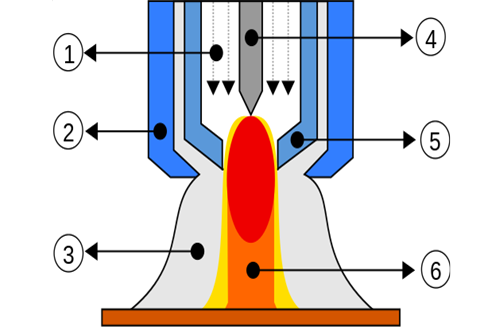
\includegraphics[width=\textwidth]{gorseller/ptaTorc}
\caption{PTA Torç}\label{fig:PtaTorc1}
\end{figure}
\lipsum[1-2]
\begin{table}
\centering
\caption{Deneme Tablosu.}\label{tab:den1}
\begin{tabular}{|l|l|l|}
\hline
sıra   & sayı   & toplam \\ \hline
1      & 2      & 3      \\ \hline
Kelime & deneme & son    \\ \hline
\end{tabular}
\end{table}

Teorem yazmak isterseniz:
\begin{theorem}[Öklid]
 İki noktadan bir ve yalnız bir doğru geçer.
\end{theorem}

İspat yazmak isterseniz:
\begin{ispat}[Tezin en önemli ispatı]
x=10
\end{ispat}

\subsubsection{Sonuçlar ve Öneriler dördüncü derece başlık}
\lipsum[1-2]
\begin{figure}[h]
\centering
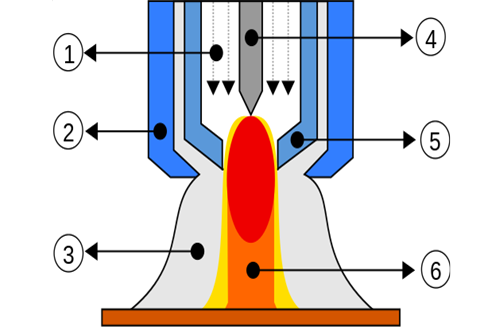
\includegraphics[width=\textwidth]{gorseller/ptaTorc}
\caption{PTA Torç}\label{fig:PtaTorc1}
\end{figure}
\lipsum[1-2]
\begin{table}
\centering
\caption{Deneme Tablosu.}\label{tab:den1}
\begin{tabular}{|l|l|l|}
\hline
sıra   & sayı   & toplam \\ \hline
1      & 2      & 3      \\ \hline
Kelime & deneme & son    \\ \hline
\end{tabular}
\end{table}

Teorem yazmak isterseniz:
\begin{theorem}[Öklid]
 İki noktadan bir ve yalnız bir doğru geçer.
\end{theorem}

İspat yazmak isterseniz:
\begin{ispat}[Tezin en önemli ispatı]
x=10
\end{ispat}

\newpage
\begin{thebibliography}{9}

\bibitem{adiv5}
ARM.(08 August 2013) ARM Debug Interface Architecure Specification [Online]

Available: https://static.docs.arm.com/ihi0031/c/IHI0031C\_debug\_interface\_as.pdf

\bibitem{git}
Micah Elizabeth Scott.(14 December 2015) esp8266-arm-swd [Online]

Available: https://github.com/scanlime/esp8266-arm-swd/blob/master/\\arm\_debug.cpp
\end{thebibliography}

%\printbibliography[title={KAYNAKLAR\space DİZİNİ}] %numaralı olsun istersen optionlarda heading=bibnumbered, yaz
%\defbibheading{bibliography}[\refname]{%
%  \section*{#1}%
%  \markboth{\MakeUppercase{#1}}{\MakeUppercase{#1}}}
%
%\addcontentsline{toc}{chapter}{\textbf{Özgeçmiş}}   % Sadece doktora tezleri için

\backmatter

\chapter{ÖZGEÇMİŞ}

Çağatay YILMAZ 1996 yılında Afyon'da doğdu. İlk, orta ve lise öğrenimini Denizli'de tamamladı. 2019 yılında Pamukkale Üniversitesi Mühendislik Fakültesi Elektrik-Elektronik Mühendisliği Bölümü'nden mezun olarak lisans öğrenimini tamamladı.

\end{document}
